\chapter{Methodology}
\label{chapter:methodology}

This section describes, in detail, the methodology behind this dissertation's research objectives, namely:

\begin{itemize}
    \item The software stack used to describe the experiments in code;
    \item The computational resources used to execute said experiments;
    \item The experiments' steps, settings, parameters, and conditions.
\end{itemize}

\section{Hardware}

Initially, computational resources from \ac{IEETA} were used in very early exploratory research:

\begin{itemize}
    \item Intel® Xeon® Processor E5-2640;
    \item NVIDIA Tesla K40c;
    \item NVIDIA Quadro K4000;
    \item 32GB DDR4 RAM.
\end{itemize}

However, given that it was shared between dozens of other researchers it was deemed not enough for a comfortable and flexible workflow because:

\begin{itemize}
    \item the little amount of memory almost wasn't enough to load the dataset into memory, especially during critically busy times;
    \item the NVIDIA Quadro K4000, with a compute capability of 3.0, was unsupported by the software stack which required a minimum compute capability of 3.7, leaving only a single NVIDIA Tesla K40c to work with.
\end{itemize}

More recently, \ac{LAR}, located in the Department of Mechanical Engineering at the University of Aveiro, has provided access to their deep learning research server codenamed Deeplar:

\begin{figure}[ht]
    \centering
    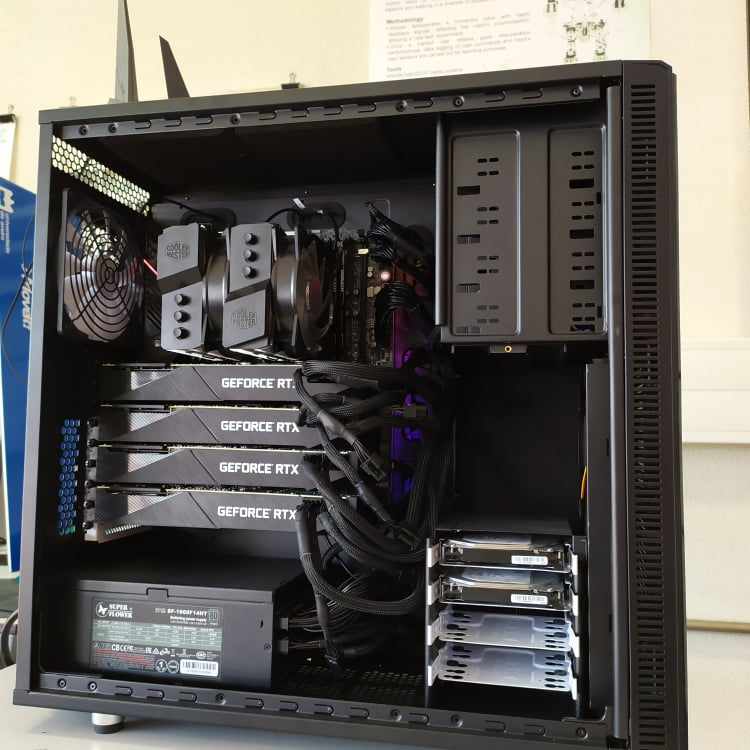
\includegraphics[width=0.6\textwidth]{figs/deeplar.jpg}
    \caption{Deeplar, the deep learning research server at \ac{LAR}}
    \label{fig:deeplar}
\end{figure}

\begin{itemize}
    \item AMD Ryzen™ Threadripper 2950X;
    \item Four NVIDIA GEFORCE® RTX 2080 Ti;
    \item 128GB DDR4 RAM.
\end{itemize}

The latter much more capable server (four state-of-the-art consumer \ac{GPU} and lots of \ac{RAM}) was effectively responsible for running this work's experiments.

\section{Software}

The deep learning research server Deeplar runs on openSUSE Tumbleweed 20191004\footnote{\url{https://software.opensuse.org/distributions/tumbleweed}}, a popular rolling-release GNU/Linux distribution. For interfacing with the \ac{GPU} it has installed CUDA 9.2 \footnote{\url{https://developer.nvidia.com/cuda-zone}} (NVIDIA GPU's proprietary language and API) and cuDNN 7.6.0 \footnote{\url{https://developer.nvidia.com/cudnn}} (a library for working with deep neural networks which most higher level frameworks rely on).

We used Miniconda\footnote{\url{https://docs.conda.io/en/latest/miniconda.html}} to install Conda\footnote{\url{https://conda.io/en/latest/}} which was used to manage a Python 3.6 \footnote{\url{https://www.python.org/}} environment which was specifically required for compatibility with TensorFlow. Crucially, the following Python packages and specific versions were used for the development of most of the source code.

\begin{itemize}
    \item TensorFlow \footnote{\url{https://www.tensorflow.org/}} 1.12.0, of which we mostly use the \verb|tf.keras| API, for training and testing the various models;
    \item scikit-learn \footnote{\url{https://scikit-learn.org/}} 0.20.2 for some useful metrics and data splitting methods;
    \item NumPy \footnote{\url{https://numpy.org/}} 1.15.4 for various vector and matrix operations and Pillow \footnote{\url{https://pillow.readthedocs.io/en/stable/}} 5.4.1 for image handling and transformations because of this work's image preprocessing needs.
\end{itemize}

\section{Data}

In a first approach we considered the ISIC 2017: Skin Lesion Analysis Towards Melanoma Detection grand challenge datasets \cite{isic2017} which provide a training set with 2000 samples (divided into three classes: 374 melanoma, 254 seborrheic keratosis, and 1372 nevus), a validation set with 150 samples, and a test set with 600 samples. However training deep neural networks for skin lesion classification requires vast amounts of high quality, reliably labeled and verified data - a set of requirements which this dataset did not meet with confidence.

The HAM10000 \cite{ham10000} dataset is an effort to boost research on automated diagnosis of dermatoscopic images that focuses on the quality and reliability of the large volume of data that is so important for successful deep learning. The extracted images (where the lesion is centered if necessary) go through an extensive semi-automatic process that filters out non-dermoscopic imaging and unreliable diagnoses, after which they are submitted to a manual review to further confirm its quality.

The datasets from the ISIC 2018 grand challenge \cite{isic2018} were largely based on HAM10000 that was already very high quality, which meant the data preprocessing needs would be much lower compared to the previous years' editions where all these quality guarantees had to be independently ensured by the competitors.

The training set is available for direct download, but the validation and test sets are kept private by the organization and are only used internally for reporting performance without actually releasing the data itself. As such, we split the samples from the training set (which is available for download) into our own training, validation and test sets.

\subsection{Preprocessing}
\label{subsection:preprocessing}

The images in the dataset undergo a number of preprocessing steps:

\begin{enumerate}
    \item Most readily available pretrained models are of network architectures whose input tensor is of square dimensions (e.g. $224 \times 224 \times 3$). Since our dataset's images are of distinct non-square dimensions, it is necessary to resize them to a square. However, resizing them all naively to the network's input tensor dimensions without regards to the image's aspect ratio means that the input fed to the network is of varying distinct aspect ratios which does not constitute a good start. Therefore, the first step is to crop an arbitrarily-sized square of the center of the image which will likely (and, in fact, does) capture the skin lesion.
    \item Resize the images to the target networks' input dimensions $224 \times 224 \times 3$ and $299 \times 299 \times 3$. We resize them as soon as possible in the data pipeline in order to reduce the computational costs of any subsequent operations on the images.
    \item Normalize the luminance and apply a 99\% contrast stretch which improves.
\end{enumerate}

\subsection{Augmentation}
\label{subsection:augmentation}

In our binary classification task (melanoma vs non-melanoma) the $m = 10015$ samples in the training set are highly imbalanced:

\begin{itemize}
    \item the majority class $S_{maj}$ constitutes 89\% of the samples;
    \item the minority class $S_{min}$ constitutes 11\% of the samples.
\end{itemize}

We correct this imbalance by oversampling the minority class, while also augmenting the total number of samples to $m' \approx 18000$ to increase the size of the dataset. That means we must augment the minority class by a factor of $\frac{\frac{m'}{2}}{|S_{min}|}$ and the majority class by a factor of $\frac{\frac{m'}{2}}{|S_{maj}|}$. For this augmentation we consider a set $T$ of possible transformations:

\begin{itemize}
    \item Horizontal flip
    \item Vertical flip
    \item 90º rotation
    \item 180º rotation
    \item 270º rotation
\end{itemize}

On principle, we did not consider transformations that change the color (e.g. contrast change, channel shift) or size (e.g. zoom) of features because it would unjustifiably allow the network to learn from these potentially misrepresenting features which even an expert human diagnosis would have trouble with.

The final available augmentations are all the $k$-combinations of the set $T$ for $k \in \{1, ..., |T|\}$, in other words all the possible ways in which you can combine the transformations from the set $T$. We end up with 17810 samples which are split 85\%-15\% (in a stratified fashion) into:

\begin{itemize}
    \item 15137 training samples
    \item 2673 test samples
\end{itemize}

The validation set is a 15\% split from the training set obtained independently at the start of each training routine (also in a stratified fashion).

\section{Experiments}

In this section we describe the methodology we followed to tackle our research question, and finally present and discuss the results.

We are skeptical of transfer learning, thus our overarching goal is to conclude whether transfer learning provides better or faster results when compared to the conventional end-to-end learning approach in which we train a network from scratch. In our search for a model for classification of skin lesions as melanoma, we will conduct experiments based on two contrasting approaches.

Within the transfer learning experiments, it is expected that extracting features from higher layers of models trained for ImageNet\cite{imagenet} classification is roughly worse than extracting features from lower layers because these provide more relevant features for skin lesion classification.

This originates a rather large number of configurations, so we use a fixed validation scheme (rather than a cross validation scheme) to minimize the computational cost. To ensure similar conditions for comparison, we set a fixed seed for every \ac{PRNG}, which in practice means parameters are initialized identically between experiments.

\begin{itemize}
    \item Binary cross entropy cost function.
    \item Train for a maximum of 1000 epochs, stopping early if the loss has not changed significantly in the last $30$ epochs.
    \item Shuffle the $m$ samples every epoch.
    \item Explicit L2 regularization with $\lambda$.
    \item Models will be evaluated and compared primarily using F1-score as measured on the test set.
\end{itemize}

\subsection{Transfer Learning Experiments}

Based on the transfer learning techniques introduced, we will explore models of VGG16, InceptionV3, and ResNet-50 architectures pre-trained on ImageNet \cite{imagenet} and transfer the weights to a new model.

\begin{enumerate}
    \item Standardize training and validation samples relative to ImageNet
    \item Mini-batch \ac{SGD} (32 samples batches) with an initial learning rate $\eta = 10^{-4}$ that decays by a factor of $10$ if the validation accuracy has not improved significantly in the last $10$ epochs
    \item Some parameters are transfered from pre-trained models and otherwise initialized according to Xavier initialization
    \item Features are extracted according to the specific experiment at hand
    \item Global average pooling to reduce the number of parameters before the classifier based on fully-connected layers
    \item Grid-search model selection based on the accuracy as measured on a fixed validation set
\end{enumerate}

% explain why vgg16, why inceptionv3, why resnet50, otherwise someone will ask me; e.g. vgg16 tratavel, da para fazer estudo exaustivo, easy to reproduce research, software libraries, replicate history

\subsubsection{VGG16}
The basic unit in traditional \ac{CNN} architectures like VGG16 is the convolutional block, which is typically comprised by a number of convolutional layers and a pooling layer at the end to sum up the convolved features. These convolutional blocks are then stacked together in the hope to progressively build higher level feature maps at the end of each block. It is possible that the features at an arbitrary convolutional layer can be used for effective transfer learning, but in some sense it is expected that the features at a pooling layer are more relevant because that was the intended design. Not only that, but considering features at arbitrary convolutional layers originates a combinatorial explosion of possible feature extractions which is just not feasible given the computational resources. As such, we will only extract features at the end of each block (i.e. from pooling layers) because it is heuristically reasonable and significantly reduces the number of layers to extract features from.

In the VGG16 architecture we are interested in extracting layers $e \in \{18,14,10,6,3\}$ and freezing layers $f \in \{18,14,10,6,3,0\}$ such that $e \geq f$ (because, obviously, one cannot freeze layers which were not extracted). When:

% TODO: maybe add ilustration, maybe refactor to background

\begin{itemize}
    \item $e = 18$ and $f = 18$ we are doing Transfer Learning by Total Feature Extraction;
    \item $e \in {14,10,6,3}$ and $f = e$ we are doing Transfer Learning by Partial Feature Extraction;

    \item $e = 18$ and $f = 0$ we are doing Transfer Learning by Total Feature Extraction and Total Fine Tuning.
    \item $e = 18$ and $f \in {14,10,6,3}$ we are doing Transfer Learning by Total Feature Extraction and Partial Fine Tuning.

    \item $e \in {14,10,6,3}$ and $f = 0$ we are doing Transfer Learning by Partial Feature Extraction and Total Fine Tuning.
    \item $e \in {14,10,6,3}$ and $f < e$ we are doing Transfer Learning by Partial Feature Extraction and Partial Fine Tuning.
\end{itemize}

Additionally, for each of these settings, we grid-search the best $\lambda$ for L2-regularization from $\lambda \in \{10^{-10}, ..., 10^{2}\}$ (spaced evenly on a log scale). This yields a total of $200$ models.


\begin{table}[ht]
\centering
\begin{tabular}{ |c|c|c|c|c|c| }
\hline
$e$ & $f$ & $\lambda$ & $A_{train}$ & $A_{val}$ & $A_{test}$ \\
\hline
18 & 18 & 100 & 0.5 & 0.5 & 0.5 \\
18 & 18 & 4.64 & 0.5 & 0.5 & 0.5 \\
18 & 18 & 0.215 & 0.748 & 0.742 & 0.528 \\
18 & 18 & 0.01 & 0.943 & 0.873 & 0.522 \\
18 & 18 & 0.000464 & 1.0 & 0.912 & 0.528 \\
18 & 18 & 2.15e-05 & 0.998 & 0.908 & 0.523 \\
18 & 18 & 1e-06 & 0.999 & 0.911 & 0.529 \\
18 & 18 & 4.64e-08 & 0.997 & 0.905 & 0.526 \\
18 & 18 & 2.15e-09 & 1.0 & 0.909 & 0.534 \\
18 & 18 & 1e-10 & 0.998 & 0.904 & 0.527 \\
18 & 14 & 100 & 0.5 & 0.5 & 0.5 \\
18 & 14 & 4.64 & 0.999 & 0.924 & 0.51 \\
18 & 14 & 0.215 & 1.0 & 0.917 & 0.505 \\
18 & 14 & 0.01 & 1.0 & 0.922 & 0.626 \\
18 & 14 & 0.000464 & 1.0 & 0.919 & 0.522 \\
18 & 14 & 2.15e-05 & 1.0 & 0.926 & 0.53 \\
18 & 14 & 1e-06 & 1.0 & 0.931 & 0.527 \\
18 & 14 & 4.64e-08 & 1.0 & 0.927 & 0.534 \\
18 & 14 & 2.15e-09 & 1.0 & 0.926 & 0.534 \\
18 & 14 & 1e-10 & 1.0 & 0.93 & 0.528 \\
18 & 10 & 100 & 0.5 & 0.5 & 0.5 \\
18 & 10 & 4.64 & 0.5 & 0.5 & 0.5 \\
18 & 10 & 0.215 & 1.0 & 0.922 & 0.526 \\
18 & 10 & 0.01 & 1.0 & 0.926 & 0.58 \\
18 & 10 & 0.000464 & 1.0 & 0.925 & 0.547 \\
18 & 10 & 2.15e-05 & 1.0 & 0.922 & 0.537 \\
18 & 10 & 1e-06 & 1.0 & 0.924 & 0.618 \\
18 & 10 & 4.64e-08 & 0.5 & 0.5 & 0.5 \\
18 & 10 & 2.15e-09 & 1.0 & 0.922 & 0.535 \\
18 & 10 & 1e-10 & 1.0 & 0.929 & 0.539 \\
18 & 6 & 100 & 0.5 & 0.5 & 0.5 \\
18 & 6 & 4.64 & 0.5 & 0.5 & 0.5 \\
18 & 6 & 0.215 & 0.5 & 0.5 & 0.5 \\
18 & 6 & 0.01 & 1.0 & 0.926 & 0.525 \\
18 & 6 & 0.000464 & 1.0 & 0.924 & 0.723 \\
18 & 6 & 2.15e-05 & 1.0 & 0.926 & 0.508 \\
18 & 6 & 1e-06 & 1.0 & 0.93 & 0.66 \\
18 & 6 & 4.64e-08 & 1.0 & 0.925 & 0.587 \\
18 & 6 & 2.15e-09 & 0.5 & 0.5 & 0.5 \\
18 & 6 & 1e-10 & 0.5 & 0.5 & 0.5 \\
18 & 3 & 100 & 0.5 & 0.5 & 0.5 \\
18 & 3 & 4.64 & 0.5 & 0.5 & 0.5 \\
18 & 3 & 0.215 & 1.0 & 0.918 & 0.582 \\
18 & 3 & 0.01 & 0.5 & 0.5 & 0.5 \\
18 & 3 & 0.000464 & 1.0 & 0.918 & 0.503 \\
18 & 3 & 2.15e-05 & 0.5 & 0.5 & 0.5 \\
18 & 3 & 1e-06 & 0.5 & 0.5 & 0.5 \\
18 & 3 & 4.64e-08 & 1.0 & 0.914 & 0.502 \\
18 & 3 & 2.15e-09 & 0.5 & 0.5 & 0.5 \\
18 & 3 & 1e-10 & 0.5 & 0.5 & 0.5 \\
18 & 0 & 100 & 0.5 & 0.5 & 0.5 \\
18 & 0 & 4.64 & 0.5 & 0.5 & 0.5 \\
18 & 0 & 0.215 & 0.5 & 0.5 & 0.5 \\
18 & 0 & 0.01 & 0.5 & 0.5 & 0.5 \\
18 & 0 & 0.000464 & 0.5 & 0.5 & 0.5 \\
18 & 0 & 2.15e-05 & 0.5 & 0.5 & 0.5 \\
18 & 0 & 1e-06 & 1.0 & 0.915 & 0.513 \\
18 & 0 & 4.64e-08 & 1.0 & 0.914 & 0.538 \\
18 & 0 & 2.15e-09 & 1.0 & 0.915 & 0.54 \\
18 & 0 & 1e-10 & 0.5 & 0.5 & 0.5 \\
14 & 14 & 100 & 0.5 & 0.5 & 0.5 \\
14 & 14 & 4.64 & 0.741 & 0.735 & 0.534 \\
14 & 14 & 0.215 & 0.804 & 0.792 & 0.504 \\
14 & 14 & 0.01 & 0.5 & 0.5 & 0.5 \\
14 & 14 & 0.000464 & 0.5 & 0.5 & 0.5 \\
14 & 14 & 2.15e-05 & 0.5 & 0.5 & 0.5 \\
14 & 14 & 1e-06 & 0.5 & 0.5 & 0.5 \\
14 & 14 & 4.64e-08 & 0.5 & 0.5 & 0.5 \\
14 & 14 & 2.15e-09 & 0.5 & 0.5 & 0.5 \\
14 & 14 & 1e-10 & 0.5 & 0.5 & 0.5 \\
14 & 10 & 100 & 0.5 & 0.5 & 0.5 \\
14 & 10 & 4.64 & 0.888 & 0.849 & 0.583 \\
14 & 10 & 0.215 & 0.5 & 0.5 & 0.5 \\
14 & 10 & 0.01 & 0.5 & 0.5 & 0.5 \\
14 & 10 & 0.000464 & 0.5 & 0.5 & 0.5 \\
14 & 10 & 2.15e-05 & 0.5 & 0.5 & 0.5 \\
14 & 10 & 1e-06 & 0.5 & 0.5 & 0.5 \\
14 & 10 & 4.64e-08 & 0.5 & 0.5 & 0.5 \\
14 & 10 & 2.15e-09 & 0.5 & 0.5 & 0.5 \\
14 & 10 & 1e-10 & 0.5 & 0.5 & 0.5 \\
14 & 6 & 100 & 0.5 & 0.5 & 0.5 \\
14 & 6 & 4.64 & 0.5 & 0.5 & 0.5 \\
14 & 6 & 0.215 & 0.5 & 0.5 & 0.5 \\
14 & 6 & 0.01 & 0.5 & 0.5 & 0.5 \\
14 & 6 & 0.000464 & 0.5 & 0.5 & 0.5 \\
14 & 6 & 2.15e-05 & 0.5 & 0.5 & 0.5 \\
14 & 6 & 1e-06 & 0.5 & 0.5 & 0.5 \\
14 & 6 & 4.64e-08 & 0.5 & 0.5 & 0.5 \\
14 & 6 & 2.15e-09 & 0.5 & 0.5 & 0.5 \\
14 & 6 & 1e-10 & 0.5 & 0.5 & 0.5 \\
14 & 3 & 100 & 0.5 & 0.5 & 0.5 \\
14 & 3 & 4.64 & 0.5 & 0.5 & 0.5 \\
14 & 3 & 0.215 & 0.5 & 0.5 & 0.5 \\
14 & 3 & 0.01 & 0.5 & 0.5 & 0.5 \\
14 & 3 & 0.000464 & 0.5 & 0.5 & 0.5 \\
14 & 3 & 2.15e-05 & 0.5 & 0.5 & 0.5 \\
14 & 3 & 1e-06 & 0.5 & 0.5 & 0.5 \\
14 & 3 & 4.64e-08 & 0.5 & 0.5 & 0.5 \\
14 & 3 & 2.15e-09 & 0.5 & 0.5 & 0.5 \\
14 & 3 & 1e-10 & 0.5 & 0.5 & 0.5 \\
14 & 0 & 100 & 0.5 & 0.5 & 0.5 \\
14 & 0 & 4.64 & 0.808 & 0.797 & 0.502 \\
14 & 0 & 0.215 & 0.5 & 0.5 & 0.5 \\
14 & 0 & 0.01 & 0.5 & 0.5 & 0.5 \\
14 & 0 & 0.000464 & 0.5 & 0.5 & 0.5 \\
14 & 0 & 2.15e-05 & 0.5 & 0.5 & 0.5 \\
14 & 0 & 1e-06 & 0.5 & 0.5 & 0.5 \\
14 & 0 & 4.64e-08 & 0.5 & 0.5 & 0.5 \\
14 & 0 & 2.15e-09 & 0.5 & 0.5 & 0.5 \\
14 & 0 & 1e-10 & 0.5 & 0.5 & 0.5 \\
10 & 10 & 100 & 0.5 & 0.5 & 0.5 \\
10 & 10 & 4.64 & 0.752 & 0.741 & 0.526 \\
10 & 10 & 0.215 & 0.768 & 0.756 & 0.502 \\
10 & 10 & 0.01 & 0.5 & 0.5 & 0.5 \\
10 & 10 & 0.000464 & 0.5 & 0.5 & 0.5 \\
10 & 10 & 2.15e-05 & 0.5 & 0.5 & 0.5 \\
10 & 10 & 1e-06 & 0.5 & 0.5 & 0.5 \\
10 & 10 & 4.64e-08 & 0.5 & 0.5 & 0.5 \\
10 & 10 & 2.15e-09 & 0.5 & 0.5 & 0.5 \\
10 & 10 & 1e-10 & 0.5 & 0.5 & 0.5 \\
10 & 6 & 100 & 0.5 & 0.5 & 0.5 \\
10 & 6 & 4.64 & 0.791 & 0.782 & 0.502 \\
10 & 6 & 0.215 & 0.5 & 0.5 & 0.5 \\
10 & 6 & 0.01 & 0.5 & 0.5 & 0.5 \\
10 & 6 & 0.000464 & 0.5 & 0.5 & 0.5 \\
10 & 6 & 2.15e-05 & 0.5 & 0.5 & 0.5 \\
10 & 6 & 1e-06 & 0.5 & 0.5 & 0.5 \\
10 & 6 & 4.64e-08 & 0.5 & 0.5 & 0.5 \\
10 & 6 & 2.15e-09 & 0.5 & 0.5 & 0.5 \\
10 & 6 & 1e-10 & 0.5 & 0.5 & 0.5 \\
10 & 3 & 100 & 0.5 & 0.5 & 0.5 \\
10 & 3 & 4.64 & 0.5 & 0.5 & 0.5 \\
10 & 3 & 0.215 & 0.5 & 0.5 & 0.5 \\
10 & 3 & 0.01 & 0.5 & 0.5 & 0.5 \\
10 & 3 & 0.000464 & 0.5 & 0.5 & 0.5 \\
10 & 3 & 2.15e-05 & 0.5 & 0.5 & 0.5 \\
10 & 3 & 1e-06 & 0.5 & 0.5 & 0.5 \\
10 & 3 & 4.64e-08 & 0.5 & 0.5 & 0.5 \\
10 & 3 & 2.15e-09 & 0.5 & 0.5 & 0.5 \\
10 & 3 & 1e-10 & 0.5 & 0.5 & 0.5 \\
10 & 0 & 100 & 0.5 & 0.5 & 0.5 \\
10 & 0 & 4.64 & 0.5 & 0.5 & 0.5 \\
10 & 0 & 0.215 & 0.5 & 0.5 & 0.5 \\
10 & 0 & 0.01 & 0.5 & 0.5 & 0.5 \\
10 & 0 & 0.000464 & 0.5 & 0.5 & 0.5 \\
10 & 0 & 2.15e-05 & 0.5 & 0.5 & 0.5 \\
10 & 0 & 1e-06 & 0.5 & 0.5 & 0.5 \\
10 & 0 & 4.64e-08 & 0.5 & 0.5 & 0.5 \\
10 & 0 & 2.15e-09 & 0.5 & 0.5 & 0.5 \\
10 & 0 & 1e-10 & 0.5 & 0.5 & 0.5 \\
6 & 6 & 100 & 0.5 & 0.5 & 0.5 \\
6 & 6 & 4.64 & 0.734 & 0.722 & 0.625 \\
6 & 6 & 0.215 & 0.746 & 0.734 & 0.587 \\
6 & 6 & 0.01 & 0.5 & 0.5 & 0.5 \\
6 & 6 & 0.000464 & 0.5 & 0.5 & 0.5 \\
6 & 6 & 2.15e-05 & 0.5 & 0.5 & 0.5 \\
6 & 6 & 1e-06 & 0.5 & 0.5 & 0.5 \\
6 & 6 & 4.64e-08 & 0.5 & 0.5 & 0.5 \\
6 & 6 & 2.15e-09 & 0.5 & 0.5 & 0.5 \\
6 & 6 & 1e-10 & 0.5 & 0.5 & 0.5 \\
6 & 3 & 100 & 0.5 & 0.5 & 0.5 \\
6 & 3 & 4.64 & 0.732 & 0.723 & 0.578 \\
6 & 3 & 0.215 & 0.821 & 0.812 & 0.5 \\
6 & 3 & 0.01 & 0.5 & 0.5 & 0.5 \\
6 & 3 & 0.000464 & 0.5 & 0.5 & 0.5 \\
6 & 3 & 2.15e-05 & 0.5 & 0.5 & 0.5 \\
6 & 3 & 1e-06 & 0.5 & 0.5 & 0.5 \\
6 & 3 & 4.64e-08 & 0.5 & 0.5 & 0.5 \\
6 & 3 & 2.15e-09 & 0.5 & 0.5 & 0.5 \\
6 & 3 & 1e-10 & 0.5 & 0.5 & 0.5 \\
6 & 0 & 100 & 0.5 & 0.5 & 0.5 \\
6 & 0 & 4.64 & 0.747 & 0.741 & 0.51 \\
6 & 0 & 0.215 & 0.798 & 0.789 & 0.5 \\
6 & 0 & 0.01 & 0.5 & 0.5 & 0.5 \\
6 & 0 & 0.000464 & 0.5 & 0.5 & 0.5 \\
6 & 0 & 2.15e-05 & 0.5 & 0.5 & 0.5 \\
6 & 0 & 1e-06 & 0.5 & 0.5 & 0.5 \\
6 & 0 & 4.64e-08 & 0.5 & 0.5 & 0.5 \\
6 & 0 & 2.15e-09 & 0.5 & 0.5 & 0.5 \\
6 & 0 & 1e-10 & 0.5 & 0.5 & 0.5 \\
3 & 3 & 100 & 0.5 & 0.5 & 0.5 \\
3 & 3 & 4.64 & 0.674 & 0.659 & 0.5 \\
3 & 3 & 0.215 & 0.5 & 0.5 & 0.5 \\
3 & 3 & 0.01 & 0.5 & 0.5 & 0.5 \\
3 & 3 & 0.000464 & 0.5 & 0.5 & 0.5 \\
3 & 3 & 2.15e-05 & 0.5 & 0.5 & 0.5 \\
3 & 3 & 1e-06 & 0.5 & 0.5 & 0.5 \\
3 & 3 & 4.64e-08 & 0.5 & 0.5 & 0.5 \\
3 & 3 & 2.15e-09 & 0.5 & 0.5 & 0.5 \\
3 & 3 & 1e-10 & 0.5 & 0.5 & 0.5 \\
3 & 0 & 100 & 0.5 & 0.5 & 0.5 \\
3 & 0 & 4.64 & 0.684 & 0.669 & 0.5 \\
3 & 0 & 0.215 & 0.722 & 0.713 & 0.5 \\
3 & 0 & 0.01 & 0.5 & 0.5 & 0.5 \\
3 & 0 & 0.000464 & 0.5 & 0.5 & 0.5 \\
3 & 0 & 2.15e-05 & 0.5 & 0.5 & 0.5 \\
3 & 0 & 1e-06 & 0.5 & 0.5 & 0.5 \\
3 & 0 & 4.64e-08 & 0.5 & 0.5 & 0.5 \\
3 & 0 & 2.15e-09 & 0.5 & 0.5 & 0.5 \\
3 & 0 & 1e-10 & 0.5 & 0.5 & 0.5 \\
\hline
\end{tabular}
\caption{Foobar}
\label{table:foobar}
\end{table}


The attained performance is subpar because the range of $\lambda$ values was not wide enough. Figures \ref{fig:results_1_18}, \ref{fig:results_1_14}, \ref{fig:results_1_10}, \ref{fig:results_1_6}, and \ref{fig:results_1_3}, plot the accuracy on the train set $A_{train}$, the accuracy on the validation set $A_{val}$, and the accuracy on the test set $A_{test}$ against the L2-regularization strength $\lambda$. It is easy to see that increasing $\lambda$ beyond that range would result in higher performance in all cases.

\begin{figure}[ht]
    \centering
    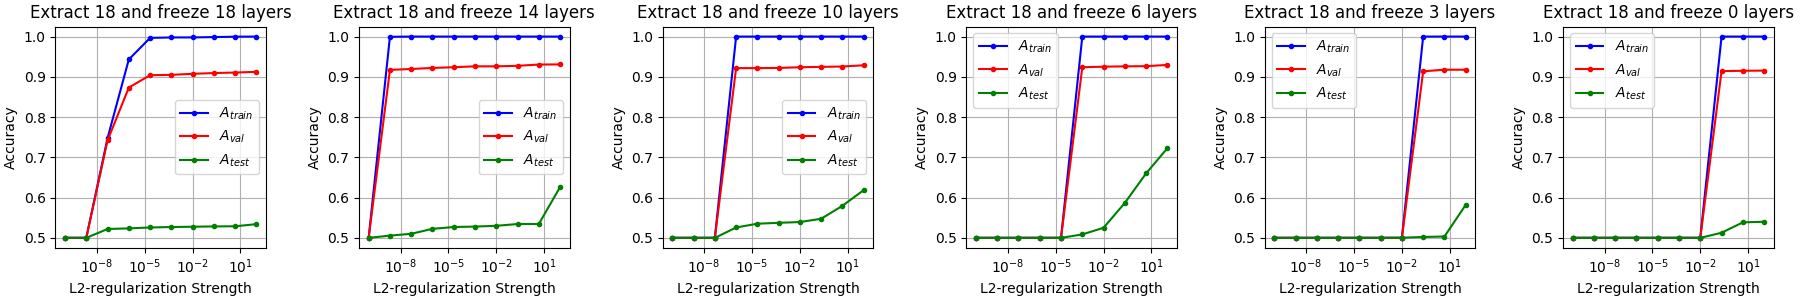
\includegraphics[width=1.0\textwidth]{figs/results_1_18.png}
    \caption{Accuracy on the train set $A_{train}$, accuracy on the validation set $A_{val}$, and accuracy on the test set $A_{test}$ against the L2-regularization strength $\lambda$ when extracting $e = 18$ layers and freezing $f \in \{18, 14, 10, 6, 3, 0\}$}
    \label{fig:results_1_18}
\end{figure}

\begin{figure}[ht]
    \centering
    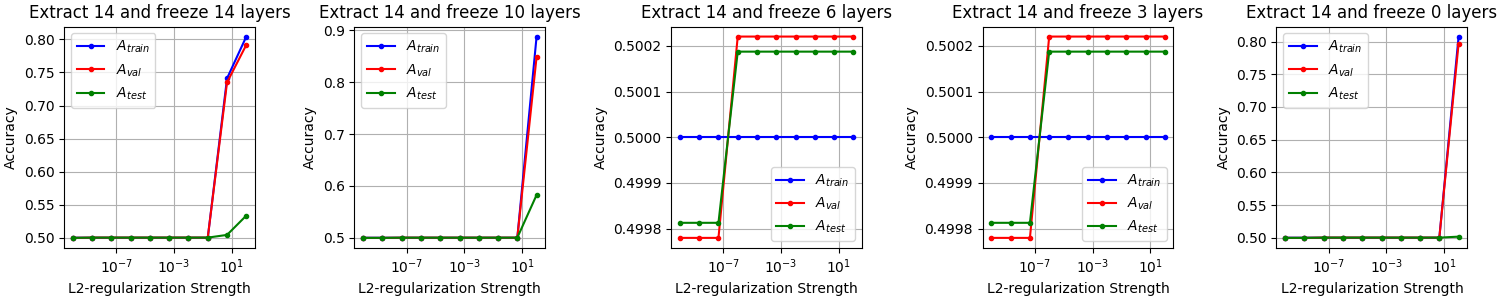
\includegraphics[width=1.0\textwidth]{figs/results_1_14.png}
    \caption{Accuracy on the train set $A_{train}$, accuracy on the validation set $A_{val}$, and accuracy on the test set $A_{test}$ against the L2-regularization strength $\lambda$ when extracting $e = 14$ layers and freezing $f \in \{14, 10, 6, 3, 0\}$}
    \label{fig:results_1_14}
\end{figure}

\begin{figure}[ht]
    \centering
    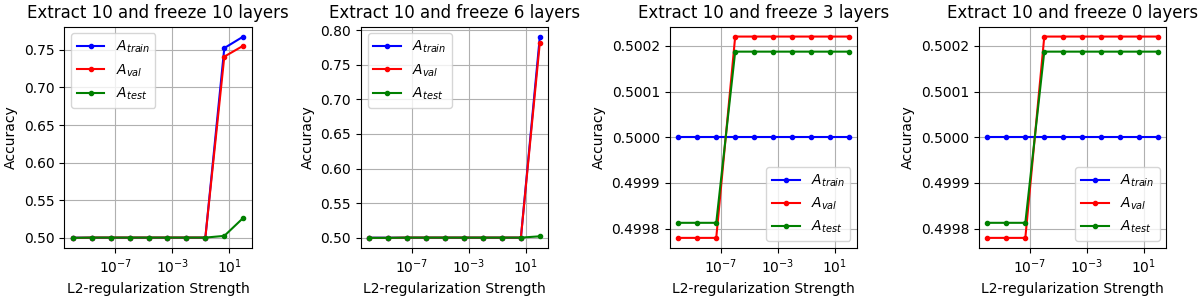
\includegraphics[width=1.0\textwidth]{figs/results_1_10.png}
    \caption{Accuracy on the train set $A_{train}$, accuracy on the validation set $A_{val}$, and accuracy on the test set $A_{test}$ against the L2-regularization strength $\lambda$ when extracting $e = 10$ layers and freezing $f \in \{10, 6, 3, 0\}$}
    \label{fig:results_1_10}
\end{figure}

\begin{figure}[ht]
    \centering
    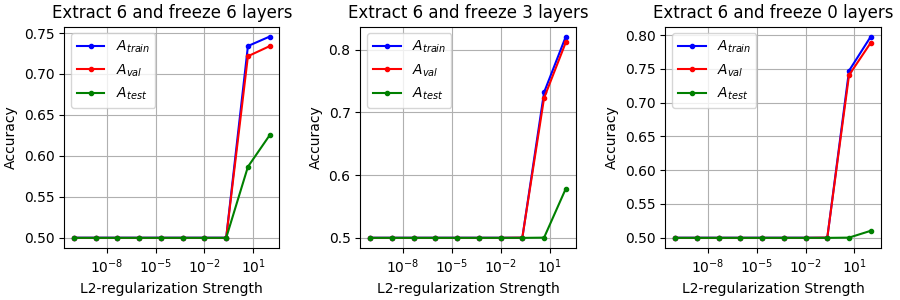
\includegraphics[width=1.0\textwidth]{figs/results_1_6.png}
    \caption{Accuracy on the train set $A_{train}$, accuracy on the validation set $A_{val}$, and accuracy on the test set $A_{test}$ against the L2-regularization strength $\lambda$ when extracting $e = 6$ layers and freezing $f \in \{6, 3, 0\}$}
    \label{fig:results_1_6}
\end{figure}

\begin{figure}[ht]
    \centering
    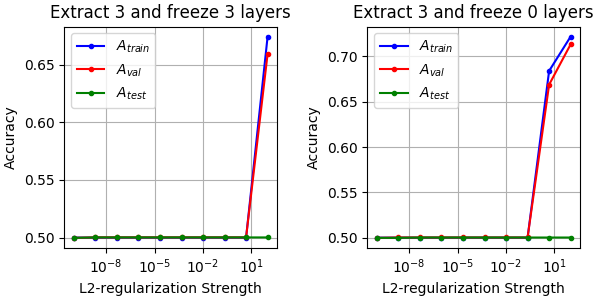
\includegraphics[width=1.0\textwidth]{figs/results_1_3.png}
    \caption{Accuracy on the train set $A_{train}$, accuracy on the validation set $A_{val}$, and accuracy on the test set $A_{test}$ against the L2-regularization strength $\lambda$ when extracting $e = 3$ layers and freezing $f \in \{3, 0\}$}
    \label{fig:results_1_3}
\end{figure}


\subsubsection{InceptionV3}

As the VGG16 experiments have shown, extracting features from higher layers yields better performance because these layers contain more useful feature maps for classification. As such, our experiments with the InceptionV3 architecture (which has hundreds more layers) will focus on these higher layers rather than exhaustively try all combinations of extracting and freezing layers.

% experiment 4
The first experiment with the InceptionV3 architecture aims to extract and freeze all layers and train a classifier on top of that.

\begin{enumerate}
    \item Extract and freeze the weights of all the convolutional layers.
    \item Connect the last layer to a global average pooling layer in order to reduce parameters before the fully-connected classifier.
    \item Connect the last layer to a fully-connected layer of 1024 ReLU-activated neurons;
    \item Connect the last layer to a fully-connected sigmoid-activated neuron for binary classification.
\end{enumerate}

Additionally, for each of these settings, we grid-search the best $\lambda$ for L2-regularization from $\lambda \in \{10^{-10}, ..., 10^{2}\}$ (spaced evenly on a log scale). This yields a total of $60$ models.

\begin{table}[ht]
\centering \begin{tabular}{ |c|c|c|c| }
\hline
lambda & train acc & val acc & test acc \\
\hline
0.0 & 0.5036 & 0.4967 & 0.5597 \\
0.0 & 0.4944 & 0.55 & 0.5373 \\
0.0651 & 0.4674 & 0.5029 & 0.4695 \\
0.0 & 0.4867 & 0.4919 & 0.4878 \\
855467.2536 & 0.4906 & 0.4963 & 0.4642 \\
0.0 & 0.5117 & 0.4914 & 0.4549 \\
0.0 & 0.4574 & 0.4337 & 0.5238 \\
0.0 & 0.4336 & 0.4919 & 0.4672 \\
0.0 & 0.536 & 0.5231 & 0.4759 \\
0.0 & 0.5105 & 0.4954 & 0.4714 \\
0.0063 & 0.4794 & 0.5328 & 0.4991 \\
0.0 & 0.4895 & 0.4861 & 0.511 \\
0.0 & 0.4859 & 0.4936 & 0.4987 \\
0.0 & 0.5281 & 0.4848 & 0.4942 \\
0.0 & 0.4923 & 0.4954 & 0.4032 \\
0.0006 & 0.5201 & 0.5324 & 0.5129 \\
92491472.7722 & 0.4841 & 0.4505 & 0.4511 \\
0.0 & 0.528 & 0.5077 & 0.4983 \\
0.0 & 0.8106 & 0.5887 & 0.4579 \\
760.9497 & 0.5173 & 0.5275 & 0.4968 \\
\hline
\end{tabular}
\caption{Foobar}
\label{table:foobar}
\end{table}

% experiment 7
Then we tried fine-tuning the top 2 inception blocks in addition to training the classifier on top of the extracted features. Like before, we grid-search the best $\lambda$ for L2-regularization from $\lambda \in \{10^{-10}, ..., 10^{2}\}$ (spaced evenly on a log scale). This yields a total of $60$ models.

\begin{table}[ht]
\centering \begin{tabular}{ |c|c|c|c| }
\hline
lambda & train acc & val acc & test acc \\
\hline
0.0 & 0.9973 & 0.5597 & 0.4833 \\
0.0 & 0.9979 & 0.5517 & 0.4901 \\
0.0 & 0.9979 & 0.5557 & 0.4901 \\
0.0063 & 0.9976 & 0.5456 & 0.4998 \\
0.0 & 0.998 & 0.5416 & 0.5039 \\
0.0 & 0.9974 & 0.5597 & 0.4991 \\
0.0 & 0.9972 & 0.5482 & 0.5006 \\
0.0 & 0.9971 & 0.5473 & 0.5013 \\
0.0 & 0.9973 & 0.5491 & 0.4972 \\
0.0 & 0.9968 & 0.5509 & 0.4991 \\
0.0 & 0.9977 & 0.5548 & 0.4998 \\
0.0 & 0.9977 & 0.5566 & 0.4998 \\
0.0 & 0.9979 & 0.5473 & 0.4987 \\
0.0 & 0.9973 & 0.5469 & 0.4994 \\
0.0 & 0.9971 & 0.561 & 0.4994 \\
0.0 & 0.9976 & 0.5592 & 0.4994 \\
0.0 & 0.9968 & 0.5504 & 0.5002 \\
0.0 & 0.9971 & 0.5557 & 0.5002 \\
0.0 & 0.9967 & 0.5553 & 0.5002 \\
0.0 & 0.9979 & 0.5619 & 0.5002 \\
\hline
\end{tabular}
\caption{Foobar}
\label{table:foobar}
\end{table}

\subsection{End-to-End Learning Experiments}

For comparison, the second set of experiments are designed to test custom architectures based around reasonable heuristics \cite{cs231n}:

\begin{itemize}
    \item The most common form of a ConvNet architecture stacks a few CONV-RELU layers, follows them with POOL layers, and repeats this pattern until the image has been merged spatially to a small size. At some point, it is common to transition to fully-connected layers.
    \item Prefer a stack of small filter convolutional layers to one large receptive field convolutional layer
    \item It is very uncommon to see receptive field sizes for max pooling that are larger than 3 because the pooling is then too lossy and aggressive. This usually leads to worse performance.
    \item Reducing sizing headaches. The scheme presented above is pleasing because all the CONV layers preserve the spatial size of their input, while the POOL layers alone are in charge of down-sampling the volumes spatially. In an alternative scheme where we use strides greater than 1 or don’t zero-pad the input in CONV layers, we would have to very carefully keep track of the input volumes throughout the CNN architecture and make sure that all strides and filters “work out”, and that the ConvNet architecture is nicely and symmetrically wired.
    \item Why use stride of 1 in CONV? Smaller strides work better in practice. Additionally, as already mentioned stride 1 allows us to leave all spatial down-sampling to the POOL layers, with the CONV layers only transforming the input volume depth-wise.
    \item Why use padding? In addition to the aforementioned benefit of keeping the spatial sizes constant after CONV, doing this actually improves performance. If the CONV layers were to not zero-pad the inputs and only perform valid convolutions, then the size of the volumes would reduce by a small amount after each CONV, and the information at the borders would be “washed away” too quickly.
\end{itemize}

In general, the models of such architectures were trained from scratch as follows:

\begin{enumerate}
    \item Standardize training and validation samples relative to ISIC2018
    \item Mini-batch \ac{SGD} (32 samples batches) with an initial learning rate $\eta = 10^{-4}$ that decays by a factor of $10$ if the validation accuracy has not improved significantly in the last $10$ epochs
    \item Parameters are all initialized according to Xavier initialization
    \item Stack convolutional and pooling layers to build useful features for classification
    \item Global average pooling to reduce the number of parameters before the classifier based on fully-connected layers
    \item Grid-search model selection based on the accuracy as measured on a fixed validation set
\end{enumerate}

\subsubsection{Custom Architecture 1}

This custom architecture stacks two convolutional layers before every pooling layer, which is a good idea for large and deep networks because multiple stacked convolutional layers can develop more complex features of the input volume before the destructive pooling operation. Specifically,

\begin{enumerate}
    \item 32 filters, 3x3 kernel, 1x1 stride, same padding, ReLU activated
    \item 32 filters, 3x3 kernel, 1x1 stride, same padding, ReLU activated
    \item 2x2 max pooling
    \item 64 filters, 3x3 kernel, 1x1 stride, same padding, ReLU activated
    \item 64 filters, 3x3 kernel, 1x1 stride, same padding, ReLU activated
    \item 2x2 max pooling
    \item 128 filters, 3x3 kernel, 1x1 stride, same padding, ReLU activated
    \item 128 filters, 3x3 kernel, 1x1 stride, same padding, ReLU activated
\end{enumerate}

The classifier is a stack of two fully-connected layers of ReLU-activated neurons followed by a fully-connected sigmoid-activated neuron for binary classification.

\begin{figure}[ht]
    \centering
    \includegraphics[width=1.0\textwidth]{figs/custom1.png}
    \caption{Architecture of the first custom-designed neural network.}
    \label{fig:custom1}
\end{figure}


\begin{table}[ht]
\centering \begin{tabular}{ |c|c|c|c|c| }
\hline
units & lambda & train acc & val acc & test acc \\
\hline
128 & 0.0 & 0.725 & 0.7222 & 0.7282 \\
128 & 0.0 & 0.725 & 0.7225 & 0.7267 \\
256 & 0.0 & 0.7214 & 0.7185 & 0.7274 \\
256 & 0.0 & 0.7215 & 0.7185 & 0.7267 \\
256 & 0.0 & 0.7215 & 0.7199 & 0.7263 \\
64 & 0.0 & 0.7225 & 0.7235 & 0.7278 \\
256 & 0.0 & 0.7213 & 0.7195 & 0.7263 \\
128 & 0.0 & 0.7237 & 0.7215 & 0.7252 \\
128 & 0.0 & 0.7237 & 0.7218 & 0.7252 \\
128 & 0.0 & 0.7237 & 0.7205 & 0.7252 \\
256 & 0.0 & 0.7221 & 0.7212 & 0.7282 \\
256 & 0.0 & 0.7228 & 0.7205 & 0.7274 \\
256 & 0.0 & 0.7211 & 0.7199 & 0.7259 \\
64 & 0.0 & 0.7232 & 0.7222 & 0.7274 \\
256 & 0.0 & 0.7222 & 0.7222 & 0.7282 \\
128 & 0.0 & 0.7238 & 0.7228 & 0.7248 \\
128 & 0.0 & 0.7241 & 0.7208 & 0.7248 \\
64 & 0.0 & 0.7213 & 0.7228 & 0.7267 \\
128 & 0.0 & 0.7241 & 0.7225 & 0.7244 \\
256 & 0.0 & 0.722 & 0.7205 & 0.7278 \\
\hline
\end{tabular}
\caption{Foobar}
\label{table:foobar}
\end{table}

\subsubsection{Custom Architecture 2}

This custom architecture uses a single convolutional layer between every pooling layer.

\begin{enumerate}
    \item 32 filters, 3x3 kernel, 1x1 stride, same padding, ReLU activated
    \item 2x2 max pooling
    \item 64 filters, 3x3 kernel, 1x1 stride, same padding, ReLU activated
    \item 2x2 max pooling
\end{enumerate}

The classifier is a single fully-connected layer of ReLU-activated neurons followed by a fully-connected sigmoid-activated neuron for binary classification.

\begin{figure}[ht]
    \centering
    \includegraphics[width=1.0\textwidth]{figs/custom2.png}
    \caption{Custom Architecture 2}
    \label{fig:custom2}
\end{figure}


\begin{table}[ht]
\centering \begin{tabular}{ |c|c|c|c|c| }
\hline
units & lambda & train acc & val acc & test acc \\
\hline
64 & 0.0 & 0.7218 & 0.7225 & 0.7368 \\
256 & 85316785.2417 & 0.6207 & 0.6135 & 0.6121 \\
64 & 0.452 & 0.6557 & 0.6574 & 0.6507 \\
512 & 0.0 & 0.5867 & 0.5834 & 0.5844 \\
512 & 52.9832 & 0.567 & 0.5804 & 0.5582 \\
128 & 727895.3844 & 0.5556 & 0.5586 & 0.547 \\
512 & 0.0 & 0.5367 & 0.5223 & 0.5343 \\
256 & 0.0 & 0.56 & 0.5441 & 0.5526 \\
256 & 10000000000 & 0.5437 & 0.5401 & 0.5343 \\
128 & 0.0 & 0.5416 & 0.5355 & 0.5256 \\
256 & 0.0 & 0.5745 & 0.5775 & 0.5747 \\
512 & 0.452 & 0.5118 & 0.5173 & 0.5313 \\
128 & 0.0 & 0.4704 & 0.4698 & 0.4803 \\
512 & 0.0 & 0.4048 & 0.4093 & 0.4141 \\
1024 & 0.0 & 0.409 & 0.4116 & 0.4219 \\
2048 & 0.0 & 0.3963 & 0.4087 & 0.3987 \\
64 & 0.0039 & 0.3674 & 0.3862 & 0.3942 \\
64 & 0.0 & 0.5104 & 0.5074 & 0.5144 \\
1024 & 0.0 & 0.496 & 0.4998 & 0.5036 \\
64 & 0.0 & 0.4958 & 0.5041 & 0.4938 \\
\hline
\end{tabular}
\caption{Foobar}
\label{table:foobar}
\end{table}

\subsection{Discussion}

Overall comparison and brief discussion after presenting results.
